\subsection{Implementing a test Service} \label{sec:testService}
To test the Kubernetes setup a simple go microservice called \textit{hello} is deployed. It listens on port 3000 and has three endpoints \textit{/hello/}, \textit{/hello/info} and \textit{/hello/path}. They don't implement any deeper logic but pose as an exemplary implementation for future services. Exemplary Kubernetes configuration files are shown and used to explain their meaning in more detail. For easier testability with cURL the microservice is based on json and not on protobufs.

\Cref{lst:dockerfileHello} shows the Dockerfile for building the microservice.
\lstset{
numbers=left, 
basicstyle=\footnotesize,
frame = single, 
language=Pascal, 
framexleftmargin=16pt,
% captionpos=b,
xleftmargin=2.3cm,
}
\begin{lstlisting}[linewidth=13cm, caption={Dockerfile for the Hello Application},label={lst:dockerfileHello}]
FROM golang:alpine as builder
EXPOSE 3000
COPY src .
RUN adduser -D -H -u 10001 scratchuser && \
    cd /go/main && \
    CGO_ENABLED=0 GOOS=linux GOARCH=arm GOARM=7 
    go build -a -installsuffix cgo -ldflags 
    '-extldflags "-static"' -o main .

FROM scratch
COPY --from=builder /etc/ssl/certs/ /etc/ssl/certs
COPY --from=builder /go/main/main /
COPY --from=builder /etc/passwd /etc/passwd
USER scratchuser
CMD ["./main"]
\end{lstlisting}
The code is cross-compiled in a builder container, which provides an isolated and replaceable build environment, this happens in line 1--8. Line 1 takes a fresh go alpine container with the latest go version. It exposes the port 3000 for the application and copies the source code in the new container in line 2 and 3, respectively. Each new command produces a new temporary cached container, thus lines 4--8 are all concatenated in one \textit{RUN} command to keep the state between commands and save resources. It first adds a new user called \textit{scratchuser} without root privileges. Then it changes directory to where the go main file directory is and cross-compiles the application for ARMv7, line 6--8. In lines 10--15, the final image is build. Line 10 initializes a new scratch container with minimal disk and memory usage. In lines 11--13 the relevant documents are copied in the new container. This includes the certificates from certificate authorities\footnote{They are important for encrypted connections.} (11), the application binary (12) and the user password (13). Line 14 switches to the scratchuser. This user has no root privileges and can never gain system control. Lastly, the default command, which is executed on container start, to start the application is defined (15).

To see how important it is to use a scratch image as a base for memory purposes, consider \cref{fig:imageSizeComparison}. It shows the disk space of the different three images, the go alpine image (bottom), the go alpine image with source and byte code (middle), and the minimal build image (top).
\begin{figure}[h!]
    \centering
    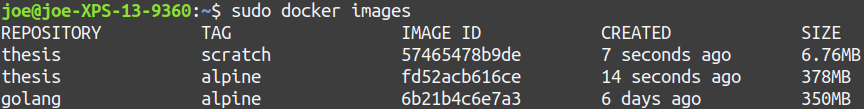
\includegraphics[scale=0.4]{figures/imageSizeComparison.png}
    \caption{The Image Sizes of Packaged Applications.}
    \label{fig:imageSizeComparison}
\end{figure}
The go alpine image is 350MB, and with source and byte code is a hefty 28MB bigger at 378MB. Copying the binary, the user files and the certificates into a scratch image takes up only 6.76MB in total. That is significantly smaller and with less overhead. When the container runs, only the binary is loaded, nothing runs in the background. In contrast, the alpine image starts a shell command line and includes an entire go build environment. 

The image is then tagged with a repository and tag name and pushed to the corresponding repository. In a short test, downloading and extracting the go alpine image on the RPi took 2:08 minutes, with 1:35 minutes spend on extracting. The scratch image with the binary only takes 0:12 seconds to download and extract.  

On the Kubernetes master, the manifest shown in \cref{lst:serviceManifest} is the service definition for the \textit{hello} application. It is an abstraction defining the guidelines how to access the pods. The service decouples the networking and the actual application from an outsiders perspective.
\lstset{
numbers=left, 
basicstyle=\footnotesize,
frame = single, 
language=Pascal, 
framexleftmargin=16pt,
% captionpos=b,
xleftmargin=2.3cm,
}
\begin{lstlisting}[linewidth=13cm, caption={The manifest of the \textit{hello} service.},label={lst:serviceManifest}]
apiVersion: v1
kind: Service
metadata:
  name: hello-service
  namespace: hello-namespace
spec:
  type: NodePort
  selector:
    app: hello
  ports:
    - name: http
      nodePort: 30001
      port: 3000
      targetPort: 3000
\end{lstlisting}
Line 5 tells the master that the service should be deployed in the namespace \textit{hello-namespace}. Line 6 specifies that each pod of this service should be accessible on the node it is scheduled on without going through the Kubernetes ingress resource. This is called nodeport and specified in line 12 to be \textit{30001}. Line 7 tells Kubernetes that the application corresponding to the service is called \textit{hello}. Finally, line 13 and 14 specify the ports the actual container expose.

For the actual state description of the application I use a \textit{Deployment} shown in \cref{lst:deploymentManifest}. A deployment specifies the desired state of the pods and the Deployment controller changes the actual state inside the cluster towards the desired state. The pods themselves are volatile and can be rescheduled by the Kubernetes control plane at any point in time. 

\lstset{
numbers=left, 
basicstyle=\footnotesize,
frame = single, 
language=Pascal, 
framexleftmargin=16pt,
escapeinside=||,
xleftmargin=2.3cm,
}
\begin{lstlisting}[linewidth=13cm, caption={The Deployment Manifest of the \textit{hello} Application.},label={lst:deploymentManifest}]
apiVersion: apps/v1
kind: Deployment
metadata:
  name: hello-deployment
  namespace: hello-namespace |\Suppressnumber|
... |\Reactivatenumber{16}|
    spec:
      affinity:
          nodeAffinity:
            requiredDuringSchedulingIgnoredDuringExecution:
              nodeSelectorTerms:
                - matchExpressions:
                    - key: kubernetes.io/hostname
                      operator: In
                      values:
                        - pihome
        podAffinity:
          requiredDuringSchedulingIgnoredDuringExecution:
            - labelSelector:
                matchExpressions:
                  - key: env
                    operator: In
                    values:
                      - test
              topologyKey: "kubernetes.io/hostname"
      nodeSelector:
        pi: "hello" 
      containers:
        - name: hello
          image: jonas27/hello:v5arm |\Suppressnumber|
...
\end{lstlisting}

\comment{
Put this in Appendix

apiVersion: apps/v1
kind: Deployment
metadata:
  name: hello-deployment
  namespace: hello-namespace
spec:
  selector:
    matchLabels:
      app: hello
  replicas: 1
  template:
    metadata:
      labels:
        app: hello
        version: v5arm
    spec:
      affinity:
          nodeAffinity:
            requiredDuringSchedulingIgnoredDuringExecution:
              nodeSelectorTerms:
                - matchExpressions:
                    - key: kubernetes.io/hostname
                      operator: In
                      values:
                        - pihome
        podAffinity:
          requiredDuringSchedulingIgnoredDuringExecution:
            - labelSelector:
                matchExpressions:
                  - key: env
                    operator: In
                    values:
                      - test
              topologyKey: "kubernetes.io/hostname"
      nodeSelector:
        pi: "hello"
      containers:
        - name: hello
          image: jonas27/hello:v5arm
          imagePullPolicy: Always
          ports:
            - containerPort: 3000

}



Line 3 and 4 specify the name and namespace of the deployment. Lines 17--34 specify the pod affinities, which places a constrained on where a certain pod can be scheduled. Similarly, anti-affinities constrain a pod to where can not be scheduled\footnote{I deployed another pod to the node beforeto satisfy the requirement}. Lines 18--25 specify a node affinity "it allows you to constrain which nodes your pod is eligible to be scheduled on, based on labels on the node"\cite{affinitiesKubernetes:online}.
Lines 26--34 specify the pod affinity. Pods of the deployment will only be scheduled on nodes containing a pod with the specified label. This enables orchestration based on other pods. Lines 35 and 36 specify the single node a deployment should be scheduled on. These three methods can be used together but have to chosen carefully. Finally, line 37--39 specify the container which should be deployed inside a pod (the port selection is hidden).

With this configuration it is possible to clearly specify the nodes a deployment should be scheduled on. However, the API resource deployments are volatile and should only be used for stateless application, like the \textit{hello} application. Stateful pods require the resource type \textit{StatefulSet} and pods supposed to run on every node require the resource type \textit{ReplicaSet}, see \cref{sec:Kubernetes} for more information.
